\documentclass{article}     
\usepackage[utf8x]{inputenc}
\usepackage[english,russian]{babel}
\usepackage[section]{placeins}
\usepackage{upgreek}
\usepackage{graphicx}
\usepackage{wrapfig}
\usepackage{amsmath}
\usepackage{epstopdf}
\graphicspath{{images/}}

\textheight 24.5cm % 29.7-2-2=25.7
\textwidth 17cm % 21-2.5-1.5=17.0
\hoffset -0.04cm %2.5-2.54=-0.04 слева 3см
\voffset -0.54cm %2-2.54=0.54 сверху 2см
\oddsidemargin 0cm
\headheight 0cm
\headsep 0cm
\topmargin 0cm


\begin{document}
\title{Градиент}
\author{   }
\date{30 июня 2017}
\maketitle

Введем сферическую систему координат, как на рисунке.

\begin{figure} [h]
    \centering
    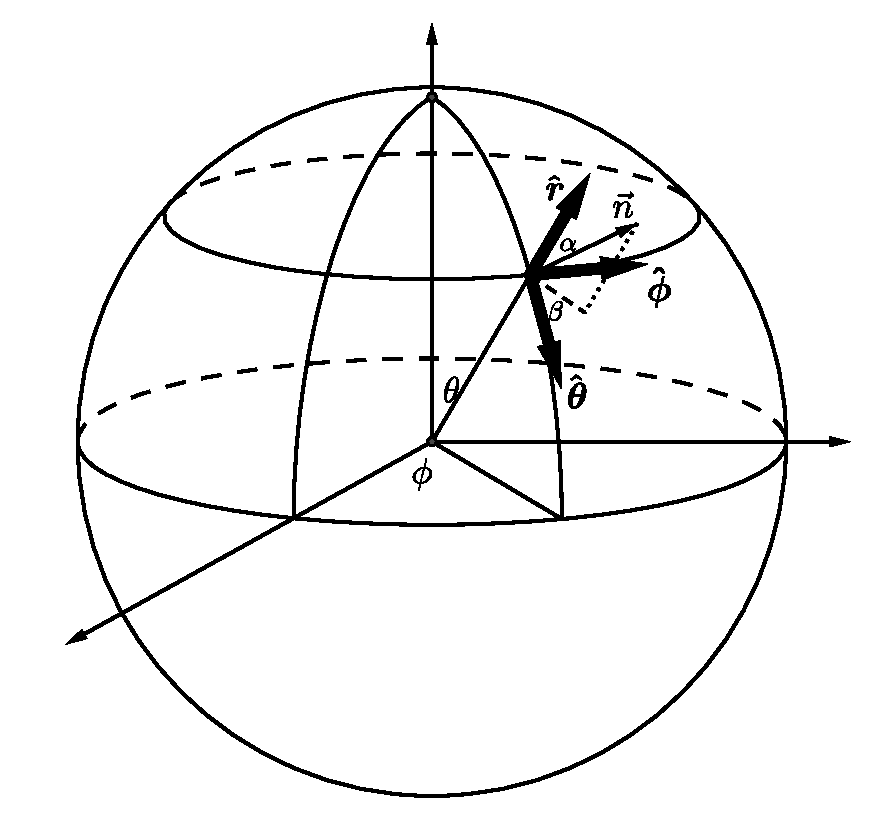
\includegraphics[scale=0.7]{Sphere2.eps}
\end{figure}

Введем в сферической системе координат вектор $\vec{n}$, направленный на наблюдателя. Распишем его по компонентно в базисе $\hat{r}, \ \hat{\theta}, \ \hat{\phi}$ в точке с координатами $r, \theta, \phi$. 

\[
\vec{n} = \lbrace \cos(\alpha), \ \frac{1}{r}\sin(\alpha)\cos(\beta), \ \frac{1}{r\sin\theta}\sin(\alpha)\sin(\beta)\rbrace
\]

Где $\cos(\alpha)$ -- косинус угла между вектором $\hat{r}$ и $\vec{n}$ (косинус полярного угла относительно $\hat{r}$), а $\cos(\beta)$ -- косинус азимутального угла $\vec{n}$, который отчитывается от $\hat{\theta}$ к $\hat{\phi}$. 
Предполагая осесиметричное движение запишем вектор скорости

\[
\vec{u} = \lbrace v^{r},\ \frac{1}{r} v^{\theta}, 0\rbrace
\]

Здесь $v^r$ -- радиальная компонента скорости, а $v^\theta$ -- тангенциальная.

Распишем скалярное произведение двух векторов в сферической системе координат

\[
\vec{u}\vec{n} = u^rn^r + r^2 u^\theta n^\theta + r^2 \sin^2\theta\ u^\phi n^\phi = u^rn^r + r^2 u^\theta n^\theta
\]

Так как здесь берется произведение двух контрвариантных векторов, то появляются коэффициенты из метрического тензора.

Чтобы взять градиент необходимо знать производные $\vec{n}$ по $r,phi,theta$. Их можно вычислить из того, что $\vec{n}$ должен быть постоянным по всему пространству, а значит его ковариантная производная равна нулю. 

\[
\nabla_l\ n^m = \frac{\partial n^m}{\partial x^l} + \Gamma^m_{kl} n^k = 0 \Rightarrow \frac{\partial n^m}{\partial x^l} = -\Gamma^m_{kl} n^k
\]

Здесь по повторным индексам производится суммирование, в котором они пробегают по буквам $r,\theta,\phi$, а $x^r, x^\theta, x^\phi$ это просто $r, \theta, \phi$. 
Запишем интересующие нас производные

\[
\begin{aligned}
\frac{\partial n^\theta}{\partial r} = -\frac{1}{r}n^\theta, \qquad \frac{\partial n^\theta}{\partial \theta} = -\frac{1}{r}n^r , \qquad \frac{\partial n^\theta}{\partial \phi} = \sin\theta\cos\theta\ n^\phi \\
\frac{\partial n^r}{\partial\theta} = rn^\theta, \qquad \frac{\partial n^r}{\partial \phi} = r\sin^2\theta\ n^\phi \\
\end{aligned}
\]

Тогда после некоторых выкладок можно получить следующее выражение для градиента по направлению $\vec{n}$


\[
\begin{aligned}
\vec{\nabla}(\vec{u}\vec{n})\vec{n} & = \frac{\partial v^r}{\partial r}\cos^2(\alpha) + \frac{1}{r}\frac{\partial v^r}{\partial \theta}\cos(\alpha)\sin(\alpha)\cos(\beta) + \frac{v^r}{r}\sin^2(\alpha) + \\
& + \frac{\partial v^{\theta}}{\partial r} \cos(\alpha)\sin(\alpha)\cos(\beta) + \frac{1}{r}\frac{\partial v^{\theta}}{\partial \theta} \sin^2(\alpha)\cos^2(\beta) - \frac{v^{\theta}}{r}\left(\cos(\alpha)\sin(\alpha)\cos(\beta) - \cot\theta\sin^2(\alpha)\sin^2(\beta)\right) \\
\end{aligned}
\] 

Стоит отметить, что при взятии второго скалярного произведения не появляются коэффициенты из метрического тензора, так как вектор градиента ($\frac{\partial}{\partial x^m}$) ковариантен, а вектор $\vec{n}$ ($n^m$) контрвариантен.

Предположим, что движение сферически симметричное. Тогда
\[
\vec{\nabla}(\vec{u}\vec{n})\vec{n} = \frac{\partial v^r}{\partial r}\cos^2(\alpha) + \frac{v^r}{r}\sin^2(\alpha)
\]

Если нет зависимости от $\theta$, и движение происходит в плоскости ($\cos(\beta) = 1$ всегда), то 


\[
\vec{\nabla}(\vec{u}\vec{n})\vec{n} = \frac{\partial v^r}{\partial r}\cos^2(\alpha) + \frac{v^r}{r}\sin^2(\alpha)+ \frac{\partial v^{\theta}}{\partial r} \cos(\alpha)\sin(\alpha) - \frac{v^{\theta}}{r}\cos(\alpha)\sin(\alpha)
\]


\end{document}